% This must be in the first 5 lines to tell arXiv to use pdfLaTeX, which is strongly recommended.
\pdfoutput=1
% In particular, the hyperref package requires pdfLaTeX in order to break URLs across lines.

\documentclass[11pt]{article}

% Remove the "review" option to generate the final version.
\usepackage{ACL2023}

% Standard package includes
\usepackage{times}
\usepackage{latexsym}
\usepackage{booktabs} % Added for \toprule, \midrule, and \bottomrule
\usepackage{amsmath} % Added for \tfrac and other math commands
\usepackage{amssymb} % Added for \mathbb and additional math symbols
\usepackage{adjustbox}
% For proper rendering and hyphenation of words containing Latin characters (including in bib files)
\usepackage[T1]{fontenc}
% For Vietnamese characters
% \usepackage[T5]{fontenc}
% See https://www.latex-project.org/help/documentation/encguide.pdf for other character sets
\usepackage{graphicx} % Added for figures
\usepackage{wrapfig}

\graphicspath{{../graphs/}{graphs/}} % Search in repo graphs/ from paper dir

% This assumes your files are encoded as UTF8
\usepackage[utf8]{inputenc}

% This is not strictly necessary, and may be commented out.
% However, it will improve the layout of the manuscript,
% and will typically save some space.
\usepackage{microtype}

% This is also not strictly necessary, and may be commented out.
% However, it will improve the aesthetics of text in
% the typewriter font.
\usepackage{inconsolata}
\usepackage{booktabs} % Added for \toprule, \midrule, and \bottomrule

\usepackage{amsmath, amssymb}
\usepackage{graphicx}
\usepackage{hyperref}
\usepackage{mathtools}
\usepackage{parskip}
\usepackage{pgfplots}
\usepackage{placeins}
\usepackage{layouts}


% If the title and author information does not fit in the area allocated, uncomment the following
%
%\setlength\titlebox{<dim>}
%
% and set <dim> to something 5cm or larger.

\title{SampledKD: Extreme Sampling, Full Distillation Accuracy}
% \title{SampledKD: How Extreme Can Sampling Be While Matching Accuracy?}
% \title{SampledKD: How Efficient Could Distillation Get While Match Accuracy?}
% \title{SampledKD: Could Distillation be So Much More Efficient?}

% Author information can be set in various styles:
% For several authors from the same institution:
% \author{Author 1 \and ... \and Author n \\
%         Address line \\ ... \\ Address line}
% if the names do not fit well on one line use
%         Author 1 \\ {\bf Author 2} \\ ... \\ {\bf Author n} \\
% For authors from different institutions:
% \author{Author 1 \\ Address line \\  ... \\ Address line
%         \And  ... \And
%         Author n \\ Address line \\ ... \\ Address line}
% To start a seperate ``row'' of authors use \AND, as in
% \author{Author 1 \\ Address line \\  ... \\ Address line
%         \AND
%         Author 2 \\ Address line \\ ... \\ Address line \And
%         Author 3 \\ Address line \\ ... \\ Address line}

\author{
  Almog Tavor\textsuperscript{*} \qquad Itay Ebenspanger\textsuperscript{*} \qquad Neil Cnaan\textsuperscript{*} \\
  Balvatnik School of Computer Science and AI \\
  Tel Aviv University \\
  \texttt{\{almogt, ebenspanger, neilcnaan\}@mail.tau.ac.il} \\
}

\begin{document}
\maketitle
\let\thefootnote\relax
\footnotemark
\footnotetext{* Equal contribution.}
\begin{abstract}
	Large language models (LLMs) achieve impressive results but are challenging to deploy due to their size and computational demands. Knowledge distillation (KD) is a popular approach for compressing LLMs, yet existing methods often suffer from efficiency-accuracy trade-offs, especially when applied to autoregressive models. We propose Entropy Knowledge Distillation (EKD), a token-selective distillation framework that leverages teacher entropy and other uncertainty measures to focus supervision on informative tokens, while maintaining unbiased class-level guidance. EKD enables efficient student training by reducing the need to store or query full teacher logits, and improves calibration and performance compared to top-$K$ truncation and other sparse KD methods. Experiments on standard language modeling benchmarks demonstrate that EKD achieves superior compression-accuracy trade-offs, paving the way for more practical deployment of compact LLMs.
\end{abstract}

\section{Introduction}

Large language models (LLMs) achieve state-of-the-art results across diverse tasks, but their size makes them expensive to serve and difficult to adapt.
Recent work shows that a small fraction of high-entropy "forking" tokens disproportionately drives learning in reinforcement learning from reasoning tasks \citep{wang2025highentropy}, suggesting that selective supervision may yield better efficiency-accuracy trade-offs.
Motivated by this insight, we study knowledge distillation (KD), a standard approach that compresses LLMs by training a smaller student model to imitate a larger teacher \citep{hinton2015distillation}, and ask whether focusing KD on these high-entropy tokens can deliver more efficient distillation without sacrificing performance.

\begin{figure}[t!]
	\begin{flushright}
		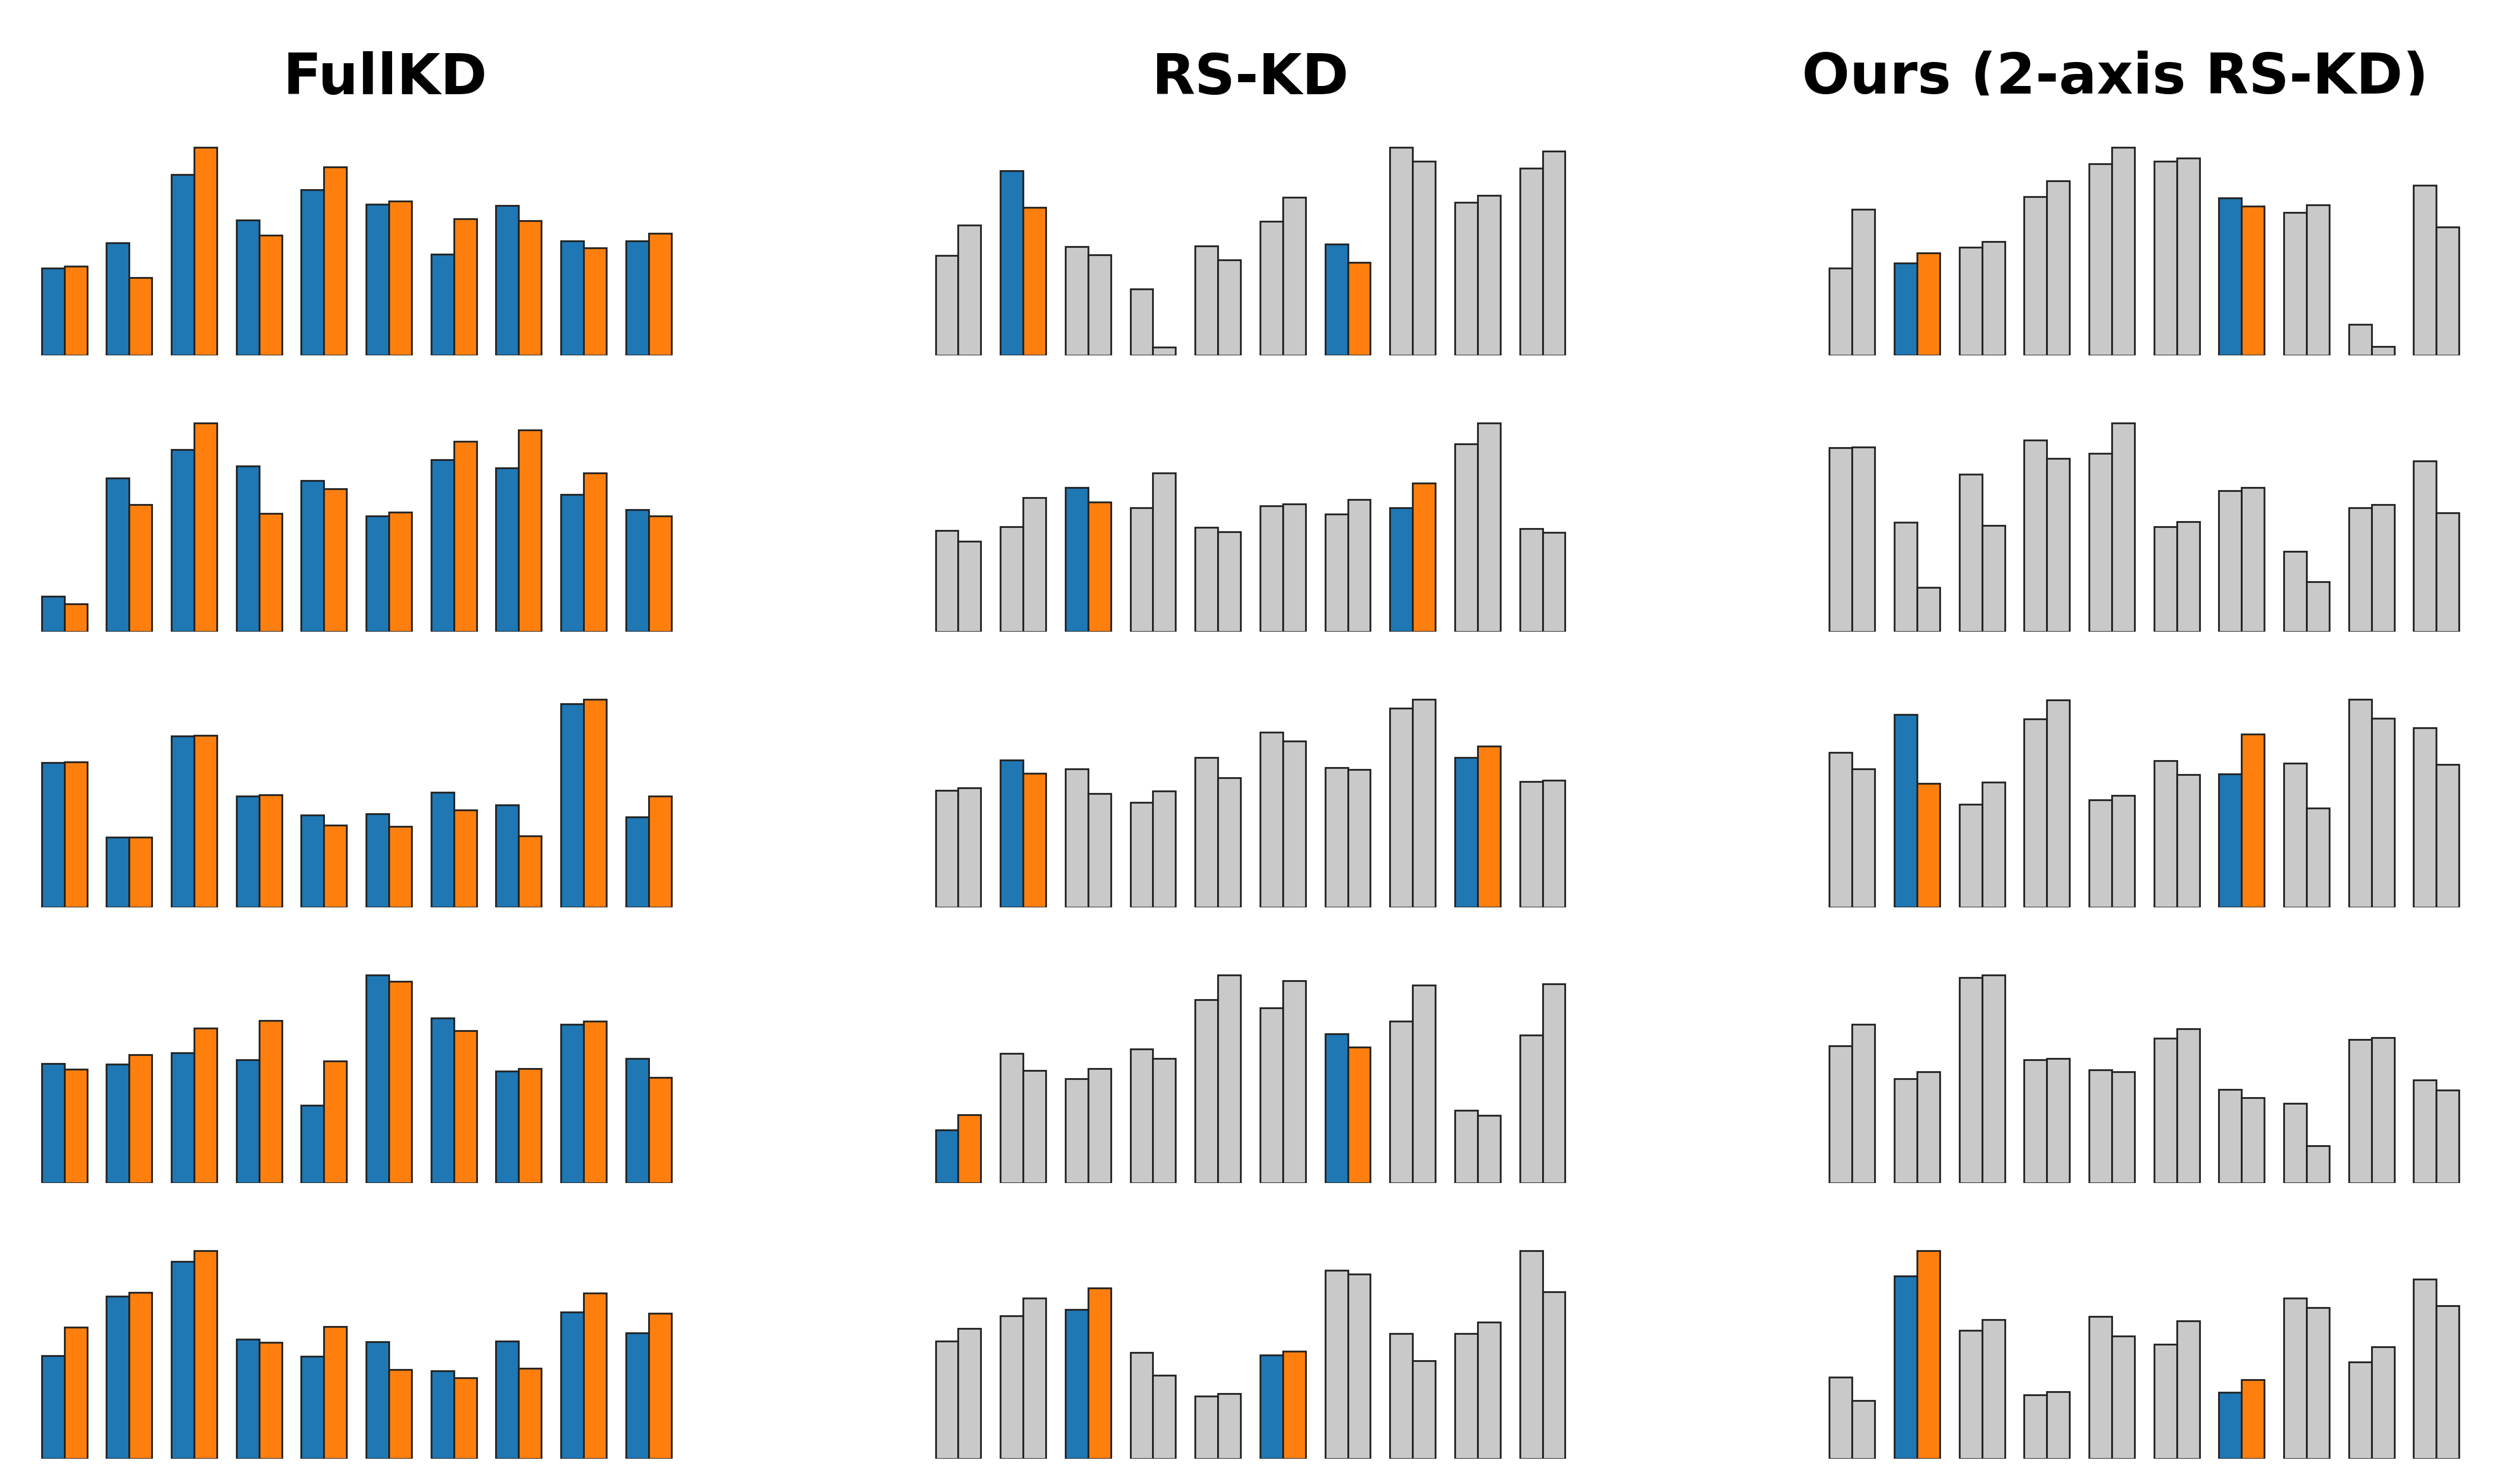
\includegraphics[width=\linewidth]{kd_intuition.png}
	\end{flushright}
	\caption{KL footprint across positions under FullKD, RS-KD, and our 2-axis scheme.}
	\label{fig:kd_intuition}
\end{figure}

While classic logit-based KD is effective for encoder-style models (e.g., DistilBERT \citep{sanh2019distilbert}), applying KD to autoregressive LLMs raises two persistent obstacles: (i) train-inference mismatch in sequence generation, and (ii) efficiency limits from storing or querying full teacher logits.

To address (i), recent work proposes on-policy distillation that trains the student on prefixes it actually produces, with the teacher scoring those prefixes \citep{agarwal2024gkd} or replacing them if uninformative (SKD) \citep{xu2024speculative}.
To address (ii), sparse alternatives avoid caching the full distribution. However, deterministic top-$K$ truncation of teacher logits (e.g., keeping only the largest $K$ probabilities) yields biased supervision and degraded calibration, especially for small $K$ \citep{anshumann2025sparse,shum2024first}.
Storing more logits improves quality but erodes the efficiency goal.

We revisit \emph{where} and \emph{how} to apply teacher supervision for LLMs.
Our thesis is that the KD budget should be spent selectively at the token level (where the teacher can add the most information) while keeping unbiased class-level supervision when it is applied.
Concretely, we:

\begin{itemize}
	\item Introduce token selective KD to allocate supervision to informative tokens using teacher entropy, teacher--student KL, or student CE. We explore various scoring functions.
	\item Use an offline teacher pass to build compact caches, then apply unbiased class sampling (RS-KD) with importance weights, matching full-KD gradients while storing only a few logits.
	\item Retain cross-entropy on all tokens for calibration and stability.
	\item Add simple curricula (increasing KD coverage) and optional EMA self-distillation.
\end{itemize}

Empirically, we compare against a range of baselines: (a) no KD, (b) full online KD on all tokens with KL divergence, (c) random token selection baselines, and (d) full Random-Sampling KD at every step \citep{anshumann2025sparse}.
Our main experiments apply token selection by teacher entropy---testing top $k\%$ thresholds across a broad sweep ($k \in \{1,2,5,10,20,\ldots,90,100\}$), as well as bucketed ranges (e.g.\ 5--15\%).
We also evaluate Top-$m$+Tail entropy approximations to reduce the computational cost of full softmax when scoring, and use the Gumbel-Max trick to sample directly from cached logits, eliminating the need to compute softmax normalization during teacher forwards.
Beyond entropy, we score tokens by alternative signals (student CE, teacher--student KL, mixtures thereof) and test curriculum schedules.
To assess robustness, we include instruction-following benchmarks.
Finally, we ablate variants such as annealed temperature, disabling CE, and an optional second phase of on-policy KD.
Our results show that token-selective, unbiased KD achieves the best accuracy--efficiency Pareto frontier while maintaining calibration.

\subsection{Contributions} (1) A unified framework for \emph{token-level} selection with unbiased class-level distillation; (2) practical scoring, curriculum, and bandit variants for allocating KD budget; (3) comprehensive evaluation vs. state-of-the-art sparse KD and selection baselines, including calibration and shift robustness.


\section{Methodology - Two-Axis Selection (SampledKD)}
\label{sec:twoaxis}
\begin{figure}[t]
	\centering
	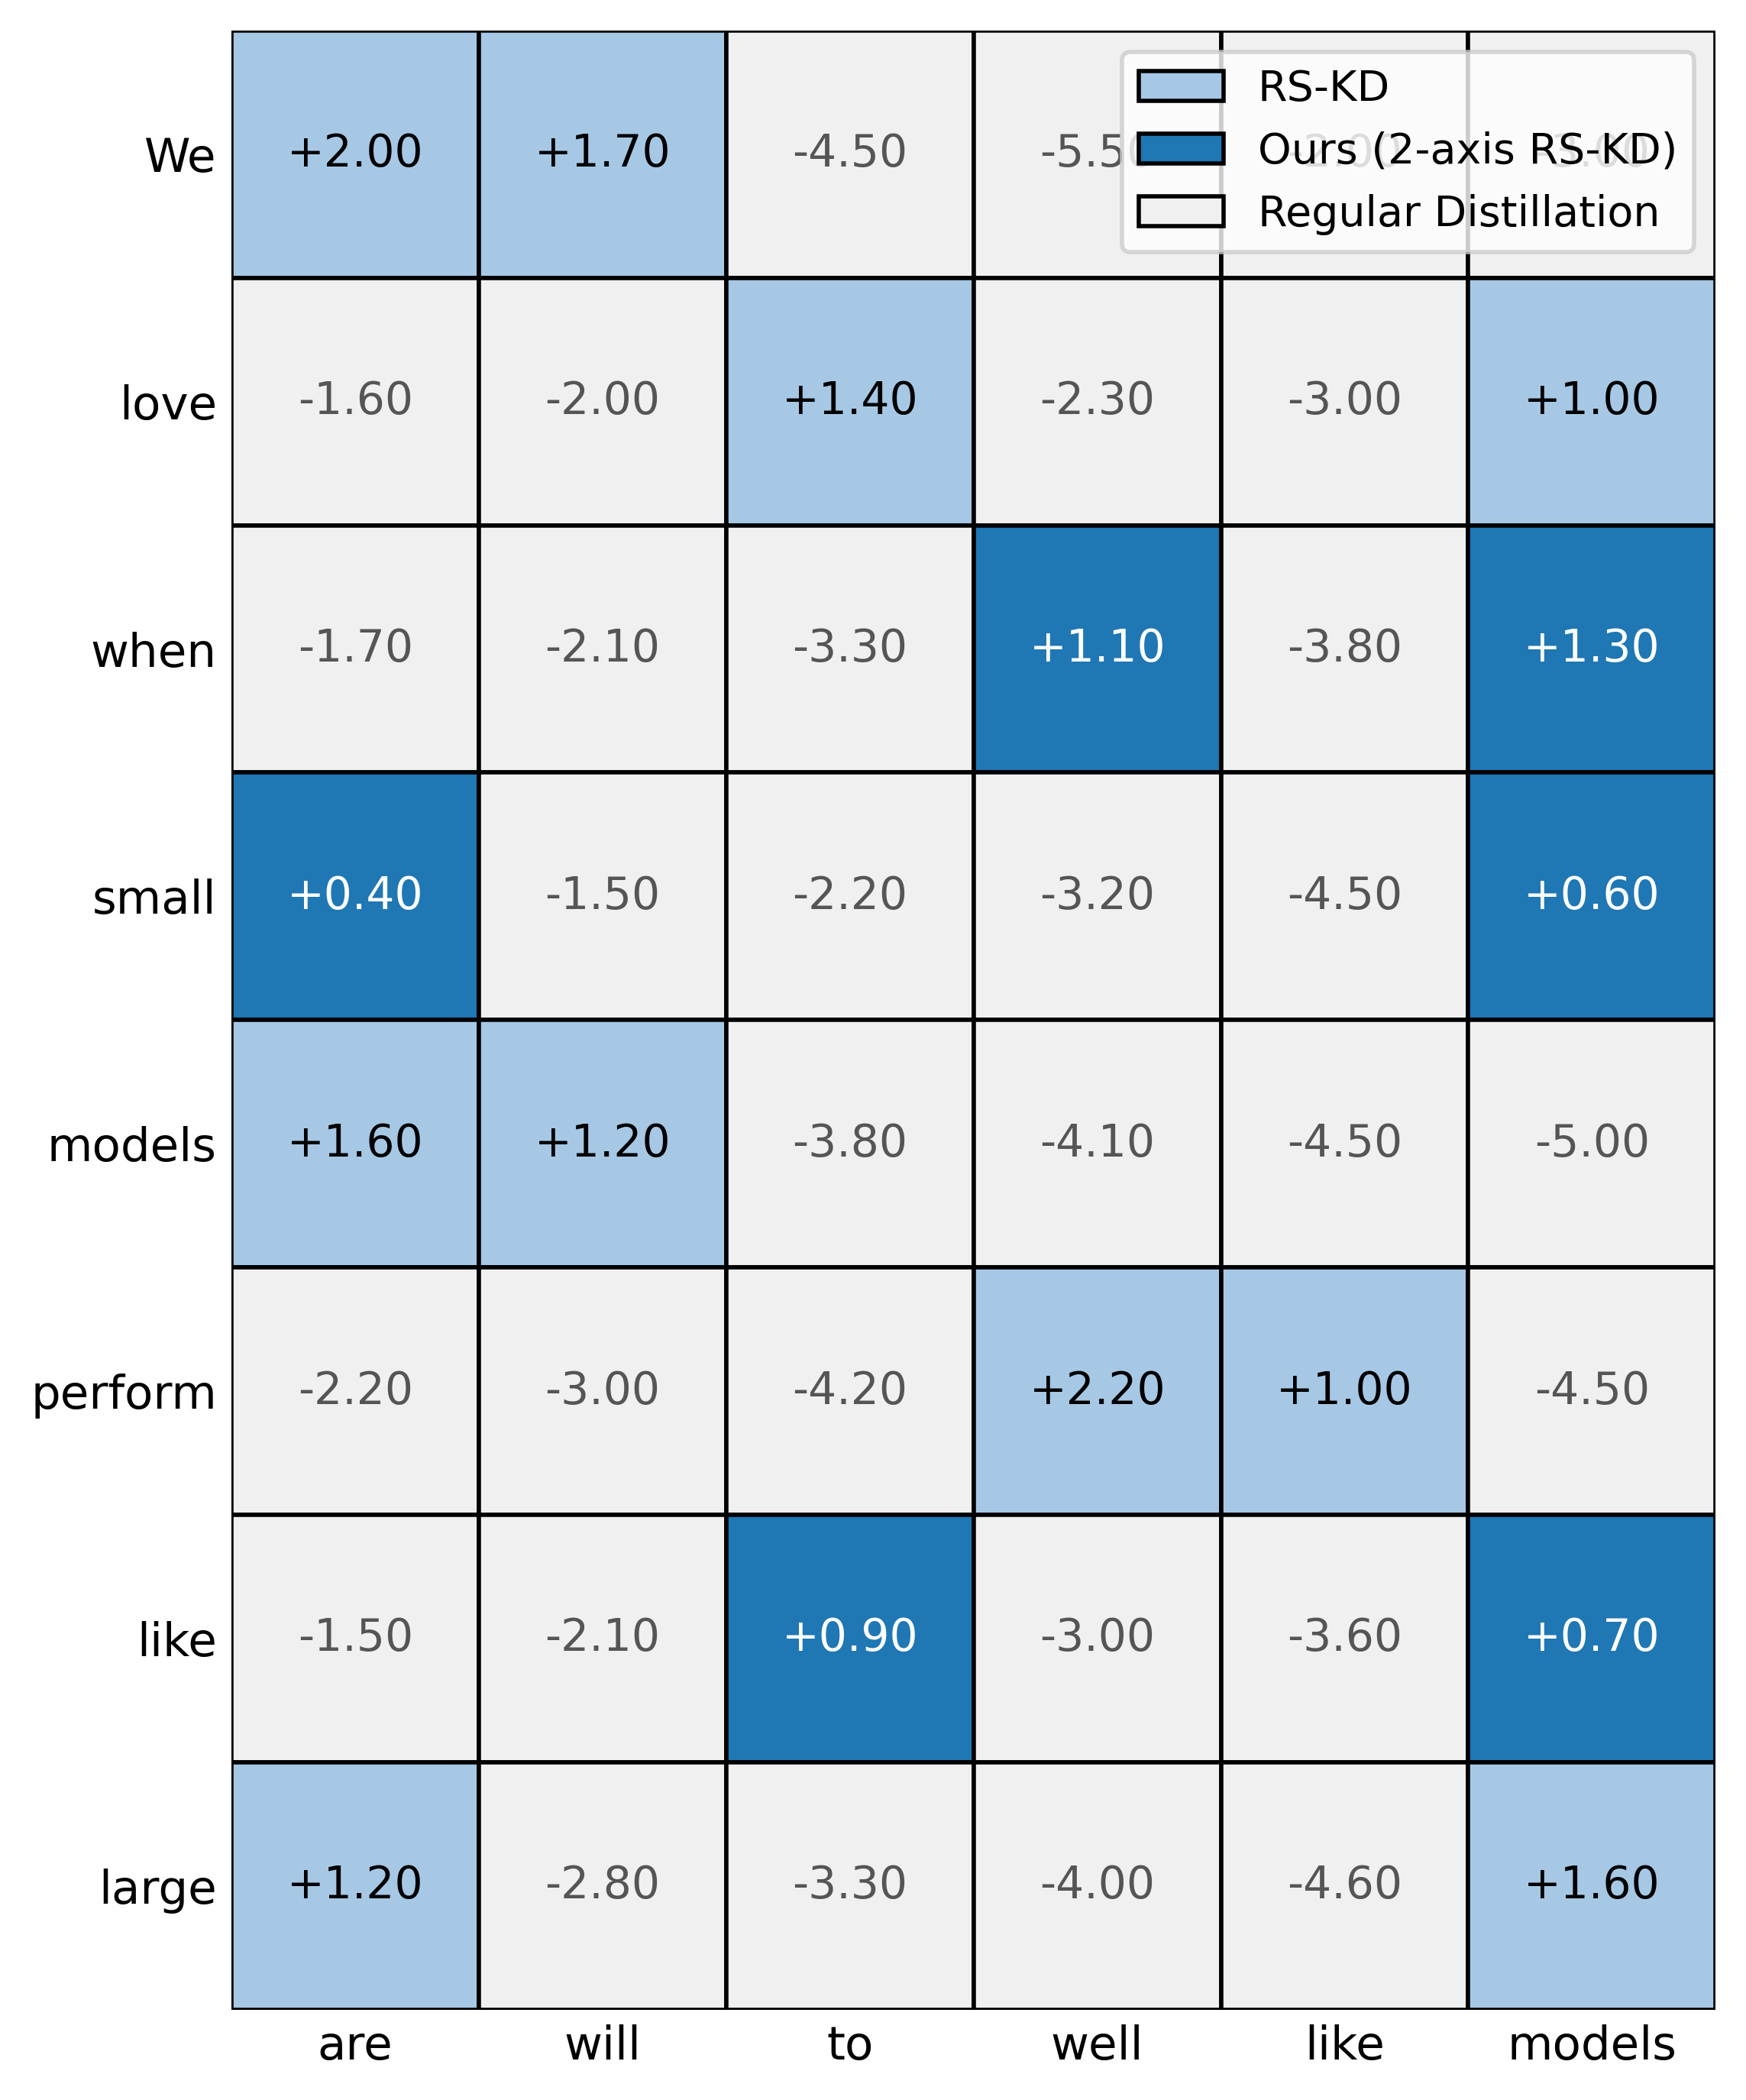
\includegraphics[width=\linewidth]{rskd_grid_two_axis_blue.png}
	\caption{Two-axis SampledKD: position-selective KD along the sequence axis (Y) and RS-KD over classes (X). Offline we cache $U$ class samples and an entropy proxy per position; online we select $K_{\text{pos}}$ positions and compute KD only over cached classes.}
	\label{fig:two-axis}
\end{figure}

\FloatBarrier

We combine (i) position-selective KD (Y axis) with (ii) RS-KD over classes (X axis) and (iii) an optimizations stack to build an efficient, unbiased estimator we call SampledKD.
Crucially, we keep the property of separating the teacher processing from student training during distillation through offline teacher cache creation.

\subsection{Offline stage (teacher forward pass, once)}
For each training sequence and position $t$:
\begin{enumerate}
	\item Compute a top-$m$ entropy proxy $H_t$ via Top-k-plus-tail (\S\ref{sec:entropy}) to drive position selection.
	\item Per position, perform RS-KD: draw $R$ samples with replacement (we optimize it via Gumbel-Max over $p_t^\tau$, where $\tau$ is temperature), compute unique IDs and counts, and retain the top-$U$ unique classes by count.
	      Convert empirical frequencies to 7-bit quantized probability $q7$.
	      %  with a residual correction to preserve normalization; pad to $U$ using a sentinel ID ($=V$).
	\item Store $(\mathcal{S}_t,\tilde p_t)$ implicitly as packed \{ID, $q7$\} pairs; $\tilde p_t$ is reconstructed at train time by normalizing the $q7$s.
\end{enumerate}
Only the packed samples and scalar $H_t$ are stored (no full logits).

\subsection{Online stage (student, many epochs)}
At each update we (i) select a subset $S$ of token positions, then (ii) compute a sampled KD loss (with optional softmax elimination) and combine it with CE.

\subsubsection{Position-selection policies}
We evaluate five policies per sequence (uniform random is a baseline):
\begin{enumerate}
	\item \textbf{Top-$k$ positions.} Select the top $K_{\text{pos}}$ positions by a score; by default the score is entropy $H_t$, and we also support a composite score that linearly combines entropy, student CE, and teacher-student KL with per-example normalization.
	\item \textbf{Percentile bucket.} Keep positions whose score lies between two percentiles (e.g., 70th-80th), filtering out both very low and very high-uncertainty tokens.
	\item \textbf{Positional RS-KD.} Instead of picking the highest-entropy positions deterministically, we sample unique positions according to a probability distribution $q_{\text{pos}}(t)\propto \big(\text{base}_t\big)^{\alpha}$. To avoid bias, each selected position is reweighted as
	      \[
		      w_t \propto  \tfrac{1}{\max(q_{\text{pos}}(t),q_{\min})},\quad \sum_{t\in S}w_t=1,
	      \]
	      so that rarely sampled tokens count more and frequent ones count less.
	\item \textbf{LinUCB bandit.} A contextual bandit model selects positions using a UCB score over per-position features (entropy, CE, KL), with a threshold and optional min/max tokens. The model is updated online with immediate rewards from distillation loss reduction.
	\item \textbf{Uniform random.} Sample $K_{\text{pos}}$ positions uniformly (baseline).
\end{enumerate}
All policies can be run with \textbf{GLS} (Global-level Selection): instead of relying solely on the current batch, we track running ranks over a global FIFO queue to approximate a global threshold (originally proposed for CE in \citet{wang2021selectivekd}); here we apply the same idea to entropy or the composite score.

\subsubsection{Loss computation (common to all policies)}
For each selected position $t$:
\begin{enumerate}
	\item \textbf{Reconstruct teacher target on cached support.} Decode the cached subset $\mathcal{S}_t$ and renormalize the stored q7 counts \emph{over $\mathcal{S}_t$} to obtain $\tilde p_t$.
	\item \textbf{Define the proposal (for sampled softmax).} If softmax elimination is enabled, augment with $M$ shared uniform negatives $\mathcal{N}_M$ and define the proposal $q_t$ \emph{over} $\mathcal{S}_t\cup\mathcal{N}_M$; normalize across this union. The teacher target $\tilde p_t$ remains supported only on $\mathcal{S}_t$.
	\item \textbf{Importance-corrected student logits.} Form
	      \[
		      \log s_t(i)\;\propto\; z_i/T \;-\; \log q_t(i).
	      \]
	\item \textbf{Sampled KD term.} Compute
	      \[
		      \mathrm{KD}_t \;=\; -\!\sum_{i\in\mathcal{S}_t} \tilde p_t(i)\,\log s_t(i).
	      \]
\end{enumerate}
Aggregate over positions and combine with CE:
\begin{align*}
	\mathcal{L} =
	 & T^2 \cdot
	\begin{cases}
		\overbrace{\sum_{t\in S} w_t\, \mathrm{KD}_t}^\text{(RS-KD with Hájek weights)} \\[2pt]
		\underbrace{\operatorname{mean}_{t\in S}\!\big[\mathrm{KD}_t\big]}_\text{(top-$k$, bucket, bandit, random)}
	\end{cases} \\
	 & +
	\alpha_{\text{ce}}\cdot \text{CE}(\text{gold},\, s).
\end{align*}
When softmax elimination is \emph{off}, CE and KD use the full-vocabulary softmax. When elimination is \emph{on}, KD uses the sampled objective above and CE uses a sampled-softmax proxy; by default CE is computed over all valid tokens, except under the bucket/random policies where we restrict CE to the selected positions to match their compute budget.

\subsection{Theoretical justification}
For a fixed position $t$, importance correction in the class-sampled softmax targets the full-vocabulary KD at temperature $T$; positional weighting ensures the aggregation recovers the uniform mean across positions. In practice we use self-normalized importance sampling and a probability floor $q_{\min}$, introducing a small bias that reduces variance and stabilizes training. Top-$k$-plus-tail provides entropy (or the composite score) at $\mathcal{O}(m)$, so both selection and class-sampling avoid any full-$V$ passes. The resulting complexity per sequence is reduced from $\mathcal{O}(N_{\text{pos}}V)$ to $\mathcal{O}(K_{\text{pos}}K_{\text{voc}})$, with $K_{\text{voc}}=|\mathcal{S}_t|{+}M$. As in standard KD, we scale the KD term by $T^2$.


\subsection{Complexity and knobs}
Compute scales as $\mathcal{O}(K_{\text{pos}}K_{\text{voc}})$ per sequence; storage is $\approx 3U + 1$ bytes per valid position (IDs+q7 plus 1-byte $\hat H$).

\subsubsection{Defaults} $U{=}12$ packed classes per position (from $R{=}50$ Gumbel draws), KD temperature $T{=}2.0$ with standard $T^2$ scaling and optional annealing, $K_{\text{pos}}\!\in\![8,32]$, $\alpha{=}1$, CE mixing $\alpha_{\text{ce}}{=}0.1$, probability floor $10^{-6}$.

\section{"Fork" Tokens Selection Variants}
\subsection{Position-Selective Distillation (RS-KD over Positions)}
\label{sec:posrs}

The KD objective for an autoregressive step is a mean over positions:
\[
	\mathcal{L}_{\text{KD}} \;=\; \frac{1}{N_{\text{pos}}} \sum_{t=1}^{N_{\text{pos}}}
	\mathrm{KL}\!\left(p_t \,\|\, s_t\right),
\]
where $p_t$ and $s_t$ are teacher and student class distributions at position $t$.
Full KD evaluates all positions; we instead sample positions using a proposal
$q_{\text{pos}}(t)$ to focus compute on informative steps while keeping the estimate (approximately) unbiased.

\subsection{Sampling rule}
We form $q_{\text{pos}}(t) \propto H_t^\alpha$ from a per-token uncertainty score $H_t$
(e.g., the Top-$k$-plus-tail lower-bound entropy from \S\ref{sec:entropy}, with $m{=}20$) and exponent $\alpha\!\ge\!0$ (higher $\alpha$ concentrates on uncertain tokens). For a sample size $K_{\text{pos}}$, the with-replacement importance-sampling estimator is
\[
	\widehat{\mathcal{L}}_{\text{KD}}^{\text{pos}} \;=\;
	\frac{1}{K_{\text{pos}}} \sum_{t \sim q_{\text{pos}}}
	\frac{1}{q_{\text{pos}}(t)} \,\mathrm{KL}\!\left(p_t \,\|\, s_t\right),
\]
which is unbiased for the uniform positional mean. We sample positions without replacement and use Hájek weights, $w_t \propto 1/q_{\text{pos}}(t)$ with $\sum_{t\in S} w_t = 1$, which yields an approximately unbiased estimate of the uniform positional mean with reduced variance.
A tiny probability floor (e.g., $10^{-6}$) stabilizes $1/q$.

\subsection{Discussion}
This \emph{position-selective} KD is orthogonal to RS-KD over classes: it reduces compute along the \emph{time/sequence} axis, not the vocabulary axis. It complements RS-KD (next section) and preserves coverage: low-uncertainty positions still contribute with nonzero probability (controlled by $\alpha$).
We keep CE on all positions for stability, and treat the position-sampled KD as an additive term.

\subsubsection{Defaults}
$\alpha{=}1$, $K_{\text{pos}}\!\in\![8,32]$, weight floor $10^{-6}$; optionally anneal $\alpha$ upward during training to shift from exploration to focused supervision.

\section{Softmax Elimination Optimizations}
\label{sec:softmax_elimination}
In a need of further efficiency boost, we eliminate full-vocabulary softmax during training, both at the teacher offline forward pass and both at the student distillation, by combining 4 optimizations.
With this change---and after batching across all valid positions with shared negatives---we improved throughput from ${\sim}2.3\text{s}/\text{step}$ to ${\sim}0.77\text{s}/\text{step}$ ($\approx3\times$ faster) on the same setup.
It is important to mention a high degradation in perplexity, dependent on hyperparameter settings.

\subsection{Student KD (importance-corrected sampled softmax)}
\label{sec:sampled_softmax}
We denote by $U_t$ the small set of cached teacher tokens per position ($|U_t|=12$).
At training time we also draw $M_t$ additional candidate tokens ($|M_t| \approx 1\text{k}$) uniformly.
Lower choices of $M_t$ have caused high perplexity degradation.
Let $S_t = U_t \cup M_t$.

For the student, we normalize its logits $z_i$ only over $S_t$ while correcting for the sampling distribution:
\[
	\hat s_t(i) = \frac{\exp(z_i/T - \log q(i))}{\sum_{j \in S_t} \exp(z_j/T - \log q(j))},
\]
where $T$ is the KD temperature.
The KD loss uses these $\hat s_t(i)$ on the cached teacher subset $U_t$. This replaces a full $\mathcal{O}(V)$ softmax with $\mathcal{O}(|S_t|)$.
The $-\log q(i)$ term yields an importance-sampling estimator whose expectation matches the full softmax \citep{jean2015large}.

\subsection{Sampled CE}
Define $\tilde z_i = z_i/T - \log q(i)$ for negatives and $\tilde z_{y_t}=z_{y_t}/T$ for the gold token (no importance correction).
Where $y_t$ is gold next-token ID at position $t$, and $i$ indexes token classes ($i\in S_t$ for KD; $i\in\{y_t\}\cup M_t$ for CE).

For the cross-entropy, we include the gold token $y_t$ and negatives $M_t$ (reused from the sampled softmax \S\ref{sec:sampled_softmax}):
\begin{align*}
	\hat s^{\text{CE}}_t(i) = \frac{\exp(\tilde z_i)}{\sum_{j \in \{y_t\}\cup M_t} \exp(\tilde z_j)},
\end{align*}
Which results
\(
\widehat{\text{CE}}_t = -\log \hat s^{\text{CE}}_t(y_t),
\)
as the sampled CE loss.
This yields an unbiased approximation to full softmax CE with cost proportional to $|M_t|$.
Prior empirical studies show that $~1k$ negatives suffice for good convergence \citep{blanc2018adaptive}.

% \section{Entropy Approximation and Gumbel Trick}
\subsection{Entropy Approximation}
\label{sec:entropy}
We estimate token uncertainty via a Top-$k$-plus-tail construction, and draw teacher samples for RS-KD via the Gumbel-Max trick---so no full softmax normalization is required during teacher forwards.
Let $u \in \mathbb{R}^V$ be teacher logits over a vocabulary of size $V$, and let
$
	p_i=\frac{e^{u_i}}{Z},\quad Z=\sum_{j=1}^V e^{u_j}
$
denote the softmax probabilities and partition function (used here only for exposition).

We compute entropy in nats (natural logarithm) and 8-bit quantization.
Order indices so that $u_{(1)} \geq \cdots \geq u_{(m)}$ are the top-$m$ logits.
Define the top-$m$ log-partition and an upper bound on the full log-partition by
\begin{align*}
	Z_m \;           & =\; \log \sum_{j \leq m} e^{u_{(j)}},           \\
	Z_{\text{ub}} \; & =\; \log\Big(e^{Z_m} + (V-m)\,e^{u_{(m)}}\Big).
\end{align*}
i.e., pessimistically setting all tail logits to $u_{(m)}$. For $j\le m$ this yields conservative probabilities:
\[
	p^{\min}_{(j)}=\exp(u_{(j)}-Z_{\text{ub}}).
\]
The remaining probability mass outside the top-$m$ is then bounded by
\begin{align*}
	\tau_{\max}=1-\sum_{j\le m}p^{\min}_{(j)},
\end{align*}
A valid lower bound on entropy $H(p)=-\sum_i p_i\log p_i$ is
\[
	H_{\text{lb}}=-\sum_{j\le m} p^{\min}_{(j)}\log p^{\min}_{(j)}\;-\;\tau_{\max}\log\tau_{\max},
\]
achieved by merging all tail mass into a single bin (coarse-graining; see \citep{cover2006elements} for background and \citep[\S3.6]{kaltchenko2025entropyheatmap} for a self-contained proof and LLM application). A corresponding upper estimate is
\[
	H_{\text{ub}}=H_{\text{lb}}+\tau_{\max}\log(V-m),
\]
(uniform tail), and the midpoint
\begin{align*}
	\widehat{H}_{\text{mid}} & =\tfrac12\!\left(H_{\text{lb}}+H_{\text{ub}}\right)                                   \\
	                         & = -\sum_{j\le m}p^{\min}_{(j)}\log p^{\min}_{(j)} \;-\; \tau_{\max}\log\tau_{\max} \; \\
	                         & \quad +\; \tfrac12\,\tau_{\max}\log(V-m).
\end{align*}

\subsection{Gumbel-Max sampling for RS-KD}
For RS-KD we require draws from the teacher distribution.
Therefore, we sample exactly from $\operatorname{softmax}(u/\tau)$ using the Gumbel-Max trick: add i.i.d.\ Gumbel noise to logits and take $\arg\max$, avoiding computation of $Z$.

\subsection{Choice of estimator and $m$}
For position ranking, $\widehat{H}_{\text{mid}}$ with $m{=}12$ gave the best accuracy-efficiency trade-off (Table~\ref{tab:entropy-ablation}).
On \texttt{GSM8K} (7{,}473 sequences; 613K tokens; 438K valid), we compared midpoint to lower/upper bounds and IS/CV-IS tail estimators (Appendix~\ref{app:tail-IS}).
Midpoint yields the best top-$k$ position overlap with exact entropy at substantially lower $m$; IS/CV-IS give the best numeric correlation, which is less relevant for selection.
Overall, entropy approximation reduces the cost of scoring positions from $\mathcal{O}(V)$ to $\mathcal{O}(m)$.
For RS-KD sampling we still require a pass over $V$ logits, but the Gumbel-Max trick avoids exponentials, normalization, and divisions, making it several times faster in wall-clock than a softmax while yielding exact samples.
Both operations are performed once in the offline teacher pass.
During training the teacher is out of the loop, and all KD terms scale only as $\mathcal{O}(K_{\text{pos}}\!\cdot\!U)$ per sequence.

\vspace{-0.5em}
\begin{table}[h]
	\centering
	\small
	\setlength{\tabcolsep}{6pt}
	\begin{tabular}{rcccccc}
		\toprule
		$m$ & \multicolumn{3}{c}{Avg. Overlap $\uparrow$} & \multicolumn{3}{c}{Avg. Corr. $\uparrow$}                                                   \\
		\cmidrule(lr){2-4}\cmidrule(lr){5-7}
		    & Mid                                         & IS                                        & CV-IS & Mid   & IS             & CV-IS          \\
		\midrule
		8   & 0.947                                       & 0.868                                     & 0.867 & 0.966 & 0.981          & 0.981          \\
		12  & 0.965                                       & 0.918                                     & 0.918 & 0.972 & 0.991          & 0.991          \\
		15  & 0.971                                       & 0.942                                     & 0.944 & 0.975 & 0.993          & 0.993          \\
		20  & \textbf{0.976}                              & 0.956                                     & 0.957 & 0.977 & \textbf{0.995} & \textbf{0.995} \\
		\bottomrule
	\end{tabular}
	\caption{GSM8K ablation ($k\%{=}20$ for position selection; Qwen3-0.6B; $s{=}5$ samples for IS/CV-IS). Midpoint attains near-peak overlap already at $m{=}12$; IS/CV-IS maximize correlation at larger $m$. (IS: importance sampling; CV-IS: control-variated IS.)}
	\label{tab:entropy-ablation}
\end{table}
\vspace{-0.75em}

\subsection{Storage accounting}
For each selected position we store $U$ sampled classes in a 24-bit word (17-bit ID, 7-bit quantized probability), plus a 1-byte entropy proxy $\hat H$ (uint8 scaled by $\ln V$).
This is $3U+1$ bytes per valid position; with $U{=}12$ this is $37$~B/token.
\[
	\text{bytes/token} = (12 \cdot 3) + 1 = 37\ \text{B/token},
\]
which yields $3.7$ TB for $N{=}10^{11}{=}100$B tokens. Compared to a vanilla RS-KD cache that keeps only the packed samples, our layout adds only \textbf{1}B for entropy per position:
\[
	\underbrace{(12 \cdot 3)}_{\text{RS-KD }=36} \;+\; \underbrace{1}_{\text{ours}}
	= 37\text{B/token}.
\]

If the selection strategy is fixed and deterministic (e.g., top-$k$ by entropy chosen offline), we can omit $\hat H$ entirely and retain only RS-KD samples at the selected positions. This slashes storage by the selection rate $k$: with $k{=}0.25$,
\begin{align*}
	\text{B}/\text{token} \; & =\; k \cdot U \cdot 3
	\;=\; 0.25 \cdot 12 \cdot 3                                                              \\
	\;                       & =\; 9~\text{B}/\text{token} \ \Longrightarrow\ 0.9~\text{TB}.
\end{align*}
We implemented this optimized layout, but retained the full cache for our ablations so that we can ablate different position-selection policies at training time without rebuilding the cache. The one-time offline preselection is straightforward and yields a major reduction when $k$ is small.
Table~\ref{tab:storage} summarizes the storage requirements across different methods.


\begin{table}[h]
	\centering
	\begin{adjustbox}{max width=\linewidth}
		\begin{tabular}{lrrr}
			\toprule
			Method                    & Entries / token          & B / entry & Total (TB)   \\
			\midrule
			Full KD                   & 100{,}000                & 1         & 10{,}000.0   \\
			Top-K 300                 & 300                      & 3         & 90.0         \\
			RS-KD (paper)             & 12                       & 3         & 3.6          \\
			\textbf{Ours (+H=1B)}     & 12                       & 3         & \textbf{3.7} \\
			\quad offline sel.~(25\%) & $12 \!\times\! 0.25 = 3$ & 3         & \textbf{0.9} \\
			Vanilla CE                & 1                        & 3         & 0.3          \\
			\bottomrule
		\end{tabular}
	\end{adjustbox}
	\caption{Cache footprint for $N{=}10^{11}{=}100\text{B}$ train tokens. RS-KD (paper) follows their packing: 17-bit vocab ID + 7-bit prob $=$ 3 B per sampled logit, 12 samples/token $\Rightarrow$ 36 B/token (3.6 TB). \textit{Ours} stores the same 12$\times$3 B plus a per-position entropy $\hat H$ in uint8 (additional 1 B/token), totaling 37 B/token (3.7 TB). The \textit{offline sel.~(25\%)} variant assumes deterministic preselection of the top-25\% positions, so $\hat H$ is omitted and storage scales by $k{=}0.25$ to $0.25{\cdot}12{\cdot}3{=}9$ B/token (0.9 TB). Totals use decimal TB, $\mathrm{TB}=\text{bytes/token}\times N/10^{12}$.}
	\label{tab:storage}
\end{table}

\section{Evaluation}
\label{sec:evaluation}

We evaluate SampledKD on a diverse set of language understanding and reasoning benchmarks to assess the effectiveness of our token-selective distillation approach. Models are pretrained on FineWeb-Edu for 1M tokens and evaluated zero-shot. All evaluations report pass@1 accuracy as the primary metric.
\subsection{Datasets}

\subsubsection{Mathematical reasoning}
\paragraph{GSM8K} \citep{cobbe2021gsm8k} contains grade-school math word problems with natural language solutions. We use the standard train/test split for distillation training and evaluation.
\paragraph{SVAMP} \citep{patel2021svamp} provides single-step arithmetic reasoning problems with algebraic variations. We leverage the available train/test split for consistent evaluation.

\subsubsection{Reading comprehension and commonsense reasoning}
\paragraph{LAMBADA (OpenAI)} \citep{paperno2016lambada} tests language models' ability to predict the final word of passages requiring broad context. Since this benchmark provides only a test set without an official training split, we use it exclusively for zero-shot evaluation.
\paragraph{HellaSwag} \citep{zellers2019hellaswag} requires selecting the most plausible continuation of everyday scenarios. We use the standard train/validation/test split.
\paragraph{PIQA} \citep{bisk2019piqa} evaluates physical commonsense reasoning through questions about everyday situations. Evaluation follows the train/validation/test split.

\subsubsection{Science and knowledge}
\paragraph{ARC-Challenge and ARC-Easy} \citep{clark2018arc} test science question answering at middle-school level, with Challenge focusing on questions requiring reasoning and Easy covering direct retrieval. Both use train/dev/test splits.

\subsubsection{Competition-level benchmarks}
\paragraph{AIME'25} evaluates mathematical reasoning on problems from the American Invitational Mathematics Examination.
\paragraph{IFEval} \citep{zhou2023ifeval} assesses instruction following through verifiable constraints.

\subsection{Experimental setup}

For benchmarks with available training splits (GSM8K, SVAMP, ARC-Challenge, ARC-Easy, HellaSwag, PIQA), we apply SampledKD during student training and evaluate on the respective test sets. For evaluation-only benchmarks (LAMBADA, AIME'25, IFEval), we assess the distilled models in a zero-shot setting to measure knowledge transfer effectiveness.

All experiments report pass@1 accuracy, measuring the percentage of problems solved correctly on the first attempt without sampling multiple outputs.

\section{Related Work}

Foundational KD \citep{hinton2015distillation} and encoder-model distillation (e.g., DistilBERT \citep{sanh2019distilbert}) have been extended to generative LMs, including sequence-level KD for neural machine translation (NMT) \citep{kim2016sequencekd}, student-to-teacher KL distillation (MiniLLM) \citep{gu2023minillm}, and on-policy distillation, where the student generates its own text and learns from the teacher's feedback, to mitigate exposure bias (GKD) \citep{agarwal2024gkd}.
More recently, cross-tokenizer distillation has been enabled by Universal Logit Distillation (ULD) \citep{boizard2024uld} and others.

\subsection{Sparse logit KD and calibration}
Deterministic top-$K$/percentile caching of teacher logits (e.g., SLIM \citep{raman2023slim} and top-$5$ variants) reduces storage but discards tail mass, inducing biased gradients and miscalibrated students.
Random-Sampling KD \citep{anshumann2025sparse} replaces truncation with importance sampling to provide unbiased gradient estimates and improved calibration.
While exploring orthogonal improvements such as CE--KLD mixing and confidence-based reweighting at the loss level, our work targets token-level selection with different confidence metrics.
Trustworthy distillation (\emph{FIRST}) focuses on calibration by processing top-$k$ vocabulary tokens with temperature scaling and label smoothing \citep{shum2024first}, whereas we apply entropy/KL-based position selection coupled with RS-KD over classes.

\subsection{Token-/word-level selective supervision} Several strands selectively apply supervision at the granularity we target. In NMT, \citet{wang2021selectivekd} select high cross-entropy \emph{words} using both batch-local and global FIFO queues (GLS). For LLM post-training, token-level uncertainty-aware learning applies masked MLE on high-uncertainty \emph{tokens} and self-distillation on the remainder to avoid OOD overfitting \citep{liu2025tokenlevel}. In continual KD, token-level cross-entropy is used to quantify when and where to distill \citep{zhang2023continualkd}. In CoT reasoning, KPOD learns token importance weights and a progressive schedule within rationales \citep{feng2024kpod}. Compared to these, our EKD selects tokens using teacher-centric uncertainty (entropy and teacher-student KL) and couples selection with \emph{unbiased} class-level Random-Sampling KD at selected positions; we also keep CE on all tokens for stability.

\subsection{Entropy/uncertainty-guided KD} Beyond selection, multiple KD variants weight supervision by uncertainty or entropy. Entropy-based adaptive KD (EA-KD) prioritizes \emph{samples} with higher entropy \citep{su2023eakd}, while DE-MKD uses teacher-prediction entropy to weight among multiple teachers \citep{cheng2024demkd}. Uncertainty-aware mixup reduces KD cost while maintaining quality \citep{xu2023unix}. Recent work also shows entropy-weighted distillation can improve reliability/calibration in classification \citep{guo2024entropykd}. Our EKD differs in using entropy/KL primarily to decide \emph{which tokens} receive external-teacher KD, not to reweight losses globally.

% (moved) Entropy approximation subsection relocated before Related Work.

\subsection{Entropy/perplexity for data selection} Selecting \emph{samples} by entropy or perplexity is long-standing in NLP. Moore-Lewis cross-entropy difference and follow-ups established perplexity-based domain selection \citep{moore2010cediff,axelrod2015few,axelrod2017cynical}. Recent LLM-scale pruning leverages perplexity or loss from small reference models \citep{ankner2024perplexedperplexityperplexitybaseddata} and surveys consolidate techniques \citep{datasel2024survey}. Active learning routinely employs entropy/margin sampling \citep{zhang2022alsurvey}. EKD is orthogonal: we operate at the token level within sequences and combine selection with unbiased sparse logits.

\subsection{Self-distillation and EMA teachers} Self-distillation regularizes students via a teacher derived from the student itself, e.g., Born-Again Networks \citep{furlanello2018ban} and Mean Teacher (EMA) consistency \citep{tarvainen2017meanteacher}. We adopt an optional EMA self-distill term as a light regularizer complementary to external-teacher KD.

\subsection{Evaluation under shift} We report in-distribution and distribution-shift results following ShiftKD \citep{zhang2023shiftkd}, which benchmarks KD methods under diversity and correlation shifts.

\subsection{Summary} Prior work either improves the \emph{where} (token/word/sample selection, curricula) or the \emph{how} (on-policy, reverse-KL, cross-tokenizer, sparse logits) of KD. We unify both: allocate KD budget to high-value tokens and deliver unbiased supervision there via Random-Sampling KD.

\bibliography{anthology, custom}
\bibliographystyle{acl_natbib}

\appendix
\section{Alternative tail estimators (unbiased IS and control variates)}
\label{app:tail-IS}
Let $T$ be the tail indices (outside top-$m$), $P_T=\sum_{v\in T}p_v$, and $q(v)=p_v/P_T$ the tail-normalized sampling distribution. The exact tail \emph{contribution to entropy} is
\[
	H_T \;=\; -\sum_{v\in T} p_v \log p_v \;=\; -P_T\,\underset{v\sim q}{\mathbb{E}}\,[\log p_v].
\]
\paragraph{Top-$m$ + naive IS} With $s$ samples $v_i\!\sim q$,
\[
	\widehat{H}_T^{\text{IS}}
	= -P_T \cdot \frac{1}{s}\sum_{i=1}^s \log p_{v_i}.
\]
\paragraph{Top-$m$ + control-variated IS (uniform baseline)}
Decompose with the uniform tail $u=\tfrac{P_T}{V-m}$:
\begin{align*}
	\sum_{v\in T} p_v \log p_v
	 & = -P_T\log\!\frac{P_T}{V-m}                                              \\
	 & + P_T\,\underset{v\sim q}{\mathbb{E}}\!\left[\log\!\frac{p_v}{u}\right].
\end{align*}
Thus, the entropy tail is
\[
	H_T^{\text{CV-IS}}
	= \underbrace{-P_T\log\!\frac{P_T}{V-m}}_{\text{baseline}}
	\;-\; P_T \cdot \underset{v\sim q}{\mathbb{E}}\!\left[\log\!\frac{p_v}{u}\right],
\]
with unbiased estimator (using $s$ samples):
\begin{align*}
	\widehat{H}_T^{\text{CV-IS}}
	 & = -P_T\log\!\frac{P_T}{V-m}                                                \\
	 & \quad - P_T \cdot \frac{1}{s}\sum_{i=1}^s \Big(\log p_{v_i} - \log u\Big).
\end{align*}
In all cases, the head contribution $H_{\text{head}}=-\sum_{j\le m}p_{(j)}\log p_{(j)}$ is computed exactly; the final estimate is $H=H_{\text{head}}+\widehat{H}_T$.

\end{document}
